\UseRawInputEncoding
\documentclass[12pt,a4paper]{article}

\usepackage[spanish]{babel}
\usepackage{listings}
\usepackage{xcolor}
\usepackage[utf8]{inputenc}
\usepackage{listingsutf8}
\usepackage[margin=2cm]{geometry}
\usepackage{graphicx}
\definecolor{lgray}{gray}{0.7}

\title{Práctica 3-Shell Scripting}
\author{Álvaro Prieto Barón}
\date{\today}


\begin{document}
\maketitle
\pagebreak
\tableofcontents
\pagebreak

\section{Ejercicio 1}
\subsection{Explicación}
\paragraph{}
El script recibe un parámetro, que debe ser la ruta de un directorio. Si no es así, imprime un mensaje de error con el uso correcto y finaliza. Cuando recibe un directorio válido, imprime el número de ficheros con extensión \textit{.c} o \textit{.h}, usando \textbf{find} y \textbf{awk}. Después imprime el número de líneas y caracteres de esos ficheros, ordenando numéricamente por el número de caracteres de mayor a menor, usando para ello las opciones -n (ordenar numéricamente) y -r (invertir orden) del comando \textbf{sort}. 

\subsection{Ejemplo de ejecución}
\paragraph{}
Uso incorrecto:
\begin{lstlisting}[basicstyle=\ttfamily\scriptsize]
$ ./ejercicio1.sh directorioInvalido
	Uso ./ejercicio1.sh <directorio>
\end{lstlisting}
\paragraph{}
Uso correcto:
\begin{lstlisting}[basicstyle=\ttfamily\scriptsize]
$ ./ejercicio1.sh ejemploCarpeta
	Hay 4 ficheros con extension .c y 5 ficheros con extension .h
	El fichero ejemploCarpeta/d1/audit.h tiene 463 lineas y 18221 caracteres
	El fichero ejemploCarpeta/d1/auditBackup.h tiene 463 lineas y 18221 caracteres
	El fichero ejemploCarpeta/d1/ecoc.h tiene 76 lineas y 2377 caracteres
	El fichero ejemploCarpeta/d1/auto_fs.h tiene 72 lineas y 2288 caracteres
	El fichero ejemploCarpeta/d1/compat.h tiene 17 lineas y 370 caracteres
	El fichero ejemploCarpeta/d2/prueba.c tiene 14 lineas y 233 caracteres
	El fichero ejemploCarpeta/d1/smo_routine.c tiene 8 lineas y 104 caracteres
	El fichero ejemploCarpeta/d1/svm_model_matlab.c tiene 6 lineas y 99 caracteres
	El fichero ejemploCarpeta/d1/d4/act_func.c tiene 5 lineas y 92 caracteres
\end{lstlisting}

\pagebreak
\section{Ejercicio 2}
\subsection{Explicación}
\paragraph{}
Recibe como parámetros el nombre de un directorio, y, opcionalmente, un umbral de tamaño. Tras comprobar si el directorio es válido y si el umbral es un número (en caso de que se haya pasado, si no ha sido especificado asigna 0), itera por todos los ficheros del directorio cuyo tamaño sea mayor que el umbral e imprime su nombre, la longitud del nombre de su propierario, la fecha de la última modificación en formato legible, la fecha del último acceso en UNIX time, su tamaño en bytes, su número de bloques, sus permisos en formato cadena y un 1 si el usuario que lanza el script tiene permisos de ejecución. 
\paragraph{}
Estos campos van separados por ";", y las líneas del resultado se ordenan de menor a mayor tamaño, usando para ello la opción -t del comando \textbf{sort}, que nos permite especificar un separador de campos distinto al espacio en blanco, por ejemplo con  \texttt{sort -t , -k 3} ordenaríamos por el tercer campo usando la coma como separador.
\paragraph{}
Para obtener la información, excepto para los dos primeros campos y para el último, usamos directamente el comando \texttt{stat}.
\subsection{Ejemplo de ejecución}

\paragraph{}
Uso incorrecto:
\begin{lstlisting}[basicstyle=\ttfamily\scriptsize]
$ ./ejercicio2.sh directorioInvalido
	Uso: ./ejercicio2.sh <directorio> [umbral]
$ ./ejercicio2.sh ejemploCarpeta estoNoEsUnNumero
	Uso: ./ejercicio2.sh <directorio> [umbral]
\end{lstlisting}
\paragraph{}
Uso correcto:
\begin{lstlisting}[basicstyle=\ttfamily\scriptsize]
$ ./ejercicio2.sh ejemploCarpeta 3000
Nombre, LongUsuario, FechaMod, FechaAcceso, Tamano, Bloques, Permisos, Ejecutable
a2.out;5-1;2016-02-28 18:09:13.000000000 +0100;1554976091;7275;16;-rwx------;1
a.out;5-1;2016-02-28 18:08:55.000000000 +0100;1554976091;7275;16;-rwx------;1
eje2;5-1;2016-02-28 18:09:34.000000000 +0100;1554976091;7275;16;-rwx------;1
centos.png;5-1;2016-02-28 18:09:16.000000000 +0100;1554976091;8215;24;-rw-------;0
pirates.jpg;5-1;2016-02-28 18:09:06.000000000 +0100;1554976091;9836;24;-rw-------;0
libhandle.so.1.0.3;5-1;2016-02-28 18:09:25.000000000 +0100;1554976092;10760;24;-rw-------;0
Linus_torvalds.jpg;5-1;2016-02-28 18:09:04.000000000 +0100;1554976091;17670;40;-rw-------;0
auditBackup.h;5-1;2017-02-24 11:46:53.000000000 +0100;1555848349;18221;40;-rw-------;0
audit.h;5-1;2017-02-24 11:46:02.000000000 +0100;1555848349;18221;40;-rw-------;0
Logo_uco.gif;5-1;2016-02-28 18:09:10.000000000 +0100;1554976091;20005;40;-rw-------;0
devocion-administrador-de-sistemas.png;5-1;2016-02-28 18:09:07.0000...[elimimado poe formato]
HD.png;5-1;2016-02-28 18:09:14.000000000 +0100;1554976091;36710;72;-rw-------;0
libsysfs.so.2;5-1;2016-02-28 18:09:29.000000000 +0100;1554976092;38644;80;-rw-------;0
richard-stallman.jpg;5-1;2016-02-28 18:09:05.000000000 +0100;1554976091;42999;88;-rw-------;0
logo_eps_grande.jpg;5-1;2016-02-28 18:09:10.000000000 +0100;1554976091;43161;88;-rw-------;0
raid0.png;5-1;2016-02-28 18:09:18.000000000 +0100;1554976091;50683;104;-rw-------;0
elinfiernoexiste.jpg;5-1;2016-02-28 18:09:02.00000000 +0100;1554976092;119847;240;-rw-------;0
libglib-2.0.so.0;5-1;2016-02-28 18:08:55.000000000 +0100;1554976092;822344;1608;-rw-------;0
\end{lstlisting}
  
\pagebreak

\section{Ejercicio 3}
\subsection{Explicación}
\paragraph{}
Este script recibe un parámetro obligatorio y dos opcionales. El primero es el nombre de un directorio, y los otros dos son dos umbrales. Tras comprobar su validez, si no hemos pasado ninguno de los opcionales, asigna  10000 y 100000. Si sólo hemos pasado uno asigna ese y 100000, usando 100000 como límite superior o inferior dependiendo del valor introducido.
\paragraph{}
Después comprueba si existen las carpetas destino, llamadas \textit{pequeños, medianos} y \textit{grandes}, si es así las borra; a continuación las crea de nuevo.
\paragraph{}
Para finalizar, clasifica los ficheros de la carpeta pasada como argumento,según su tamaño, comparándolos con los umbrales. 
\subsection{Ejemplo de ejecución}
\paragraph{}
\begin{lstlisting}[basicstyle=\ttfamily\scriptsize]
$ ./ejercicio3.sh ejemploCarpeta 20000 60000
	Los directorios destino ya existen. Borrando...
	Copiando los archivos...
$ ls pequenos
	a2.out act_func.c a.out auditBackup.h audit.h auto_fs.h bcache.cpp centos.png compat.h 
	debian.png ecoc.h eje2 ejemploSuid.sh fedora.png libhandle.so.1.0.3 Linus_torvalds.jpg 
	pirates.jpg prueba.c smo_routine.c svm_model_matlab.c
$ ls medianos
	devocion-administrador-de-sistemas.png  HD.png  libsysfs.so.2  logo_eps_grande.jpg  
	Logo_uco.gif  raid0.png  richard-stallman.jpg
$ ls grandes
	elinfiernoexiste.jpg  libglib-2.0.so.0
$ ls -l pequenos/a.out
	-rwx------ 1 adoenlunnae adoenlunnae 7,2K abr 21 19:12 pequenos/a.out*
$ ls -l medianos/HD.png
	-rw------- 1 adoenlunnae adoenlunnae 36K abr 21 19:19 medianos/HD.png
$ ls -l grandes/ elinfiernoexiste.jpg
	-rw------- 1 adoenlunnae adoenlunnae 118K abr 21 19:19 grandes/elinfiernoexiste.jpg
\end{lstlisting}
\pagebreak
\section{Ejercicio 4}
\subsection{Explicación}
\paragraph{}
El script imprime por orden alfabético los usuarios conectados, eliminando los repetidos. Para esto usa \texttt{who, awk, sort} y \texttt{uniq}.
\paragraph{}
A continuación pide un carácter por teclado, con un límite de tiempo de 5 segundos. Si no se introduce nada, se asignará el carácter 'a'. Para lograr esto usamos:
\begin{lstlisting}[basicstyle=\ttfamily\small,language=bash]
if ! read -n 1 -t 5 c;then   
        c="a"
fi  
\end{lstlisting}
Al usar un comando como condición en un \texttt{if}, entramos únicamente si la ejecución es correcta. Como hemos añadido un "!", entraremos cuando la ejecución del \texttt{read} falle, es decir, cuando no se introduzca ningún carácter. La opción -n especifica el número máximo de caracteres a leer.

\paragraph{}
Por último, el script cuenta las apariciones del carácter introducido en los nombres de ficheros y directorios dentro de la carpeta desde la que se lanza. Usa la opción \texttt{-o} de \texttt{grep}, que imprime cada aparición por separado(mientras que \texttt{grep} sin más puede imprimir en la misma línea varias si aparecen en la misma línea del fichero de entrada), y \texttt{wc -l}.

\subsection{Ejemplo de ejecución}
\begin{lstlisting}[basicstyle=\ttfamily\scriptsize,language=bash]
$ cd ejemploCarpeta && ../ejercicio4.sh
	i72prbaa
	Que caracter quieres contar?   f
El caracter 'f' aparece 6 veces en nombres de ficheros o directorios
$ ../ejercicio4.sh
	i72prbaa
	Que caracter quieres contar?
El caracter 'a' aparece 29 veces en nombres de ficheros o directorios
\end{lstlisting}
\pagebreak

\section{Ejercicio 5}
\subsection{Explicación}
\paragraph{}
El script recibe una serie de nombres de archivo y genera en \texttt{\$HOME/Copia} un archivo \textit{.tar.gz} con el nombre copia-\textbf{nombreusuario}-\textbf{fecha\_en\_unix\_time}.tar.gz . Además, borra todas los ficheros de más de 200 segundos de antigüedad de esa carpeta. El único comando nuevo que se usa es \texttt{date +\%s}, que devuelve la fecha actual en segundos.

\subsection{Ejemplo de ejecución}
\paragraph{}
\begin{lstlisting}[basicstyle=\ttfamily\small,language=bash]
$ ./ejercicio5.sh ejemploCarpeta/d1
	Copia de seguridad creada correctamente
$ tar -tf /home/i72prbaa/Copia/copia-i72prbaa-1555879566.tar.gz 
	ejemploCarpeta/d1/
	ejemploCarpeta/d1/smo_routine.c
	ejemploCarpeta/d1/compat.h
	ejemploCarpeta/d1/auditBackup.h
	ejemploCarpeta/d1/ecoc.h
	ejemploCarpeta/d1/d4/
	ejemploCarpeta/d1/d4/libsysfs.so.2
	ejemploCarpeta/d1/d4/bcache.cpp
	ejemploCarpeta/d1/d4/act_func.c
	ejemploCarpeta/d1/auto_fs.h
	ejemploCarpeta/d1/audit.h
	ejemploCarpeta/d1/svm_model_matlab.c
	ejemploCarpeta/d1/libhandle.so.1.0.3
$ ./ejercicio5.sh ejemploCarpeta/d1                  
	Borrando /home/i72prbaa/Copia/copia-i72prbaa-1555879566.tar.gz 
	de 206 segundos de antiguedad
	Copia de seguridad creada correctamente

\end{lstlisting}

\pagebreak

\section{Ejercicio 6}
\subsection{Explicación}
\paragraph{}
El script recibe el nombre de un directorio y genera un fichero html con el mismo nombre en el que se listan las carpetas y archivos que contiene.
\paragraph{}
El funcionamiento se basa en una función que se aplica recursivamente a los directorios, imprimiendo al archivo el código HTML al fichero creado anteriormente.
\subsection{Ejemplos de ejecución}
\begin{lstlisting}[basicstyle=\ttfamily\scriptsize,language=HTML]
$ ./ejercicio6.sh ejempolCarpeta
	Generando el listado en el fichero ejemploCarpeta.html
$ cat ejemploCarpeta.html
	<html>
<head>
<title>Listado del directorio ejemploCarpeta</title>
</head>
<body>
<ul>
<li><strong>/home/adoenlunnae/Uni/2o/c2/pas/p3/ejemploCarpeta/d2</strong></li>
<ul>
<li>/home/adoenlunnae/Uni/2o/c2/pas/p3/ejemploCarpeta/d2/libglib-2.0.so.0</li>
<li>/home/adoenlunnae/Uni/2o/c2/pas/p3/ejemploCarpeta/d2/prueba.c</li>
<li>/home/adoenlunnae/Uni/2o/c2/pas/p3/ejemploCarpeta/d2/ejemploSuid.sh</li>
<li>/home/adoenlunnae/Uni/2o/c2/pas/p3/ejemploCarpeta/d2/a.out</li>
</ul>
<li><strong>/home/adoenlunnae/Uni/2o/c2/pas/p3/ejemploCarpeta/d3</strong></li>
.
.
.
.
</body>
</html>
\end{lstlisting}

\begin{figure}[h]
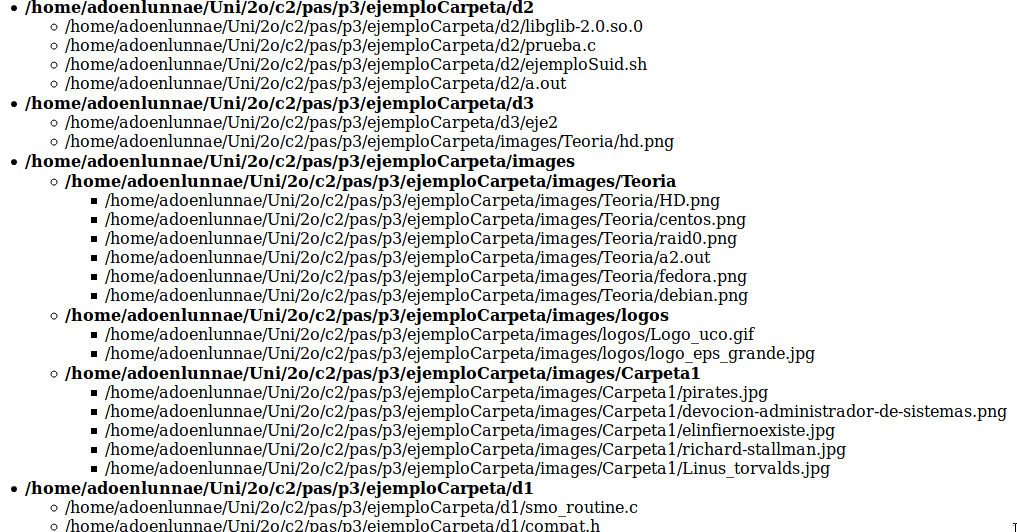
\includegraphics[width=\textwidth]{CapturaHTML.png} 
\end{figure}





\end{document}